\setbeamercolor*{title}{fg=Blue}
		\setbeamercolor*{structure}{fg=Blue}

	\setbeamercolor*{footlinecolor}{fg=white,bg=Blue}
	\setbeamertemplate{footline}{\begin{beamercolorbox}[sep=0.5em,wd=\paperwidth,ht=1.35cm,leftskip=0.5cm,rightskip=0.5cm]{footlinecolor}
\parbox{\linewidth}{\centering Engineering}
  	\end{beamercolorbox}%}
	}

	\begin{frame}
	\frametitle{\textbf{Chinmay Nivargi}}
	\begin{columns}[T]
	     \begin{column}{0.4\textwidth}
	     \centering
	       \begin{figure}
	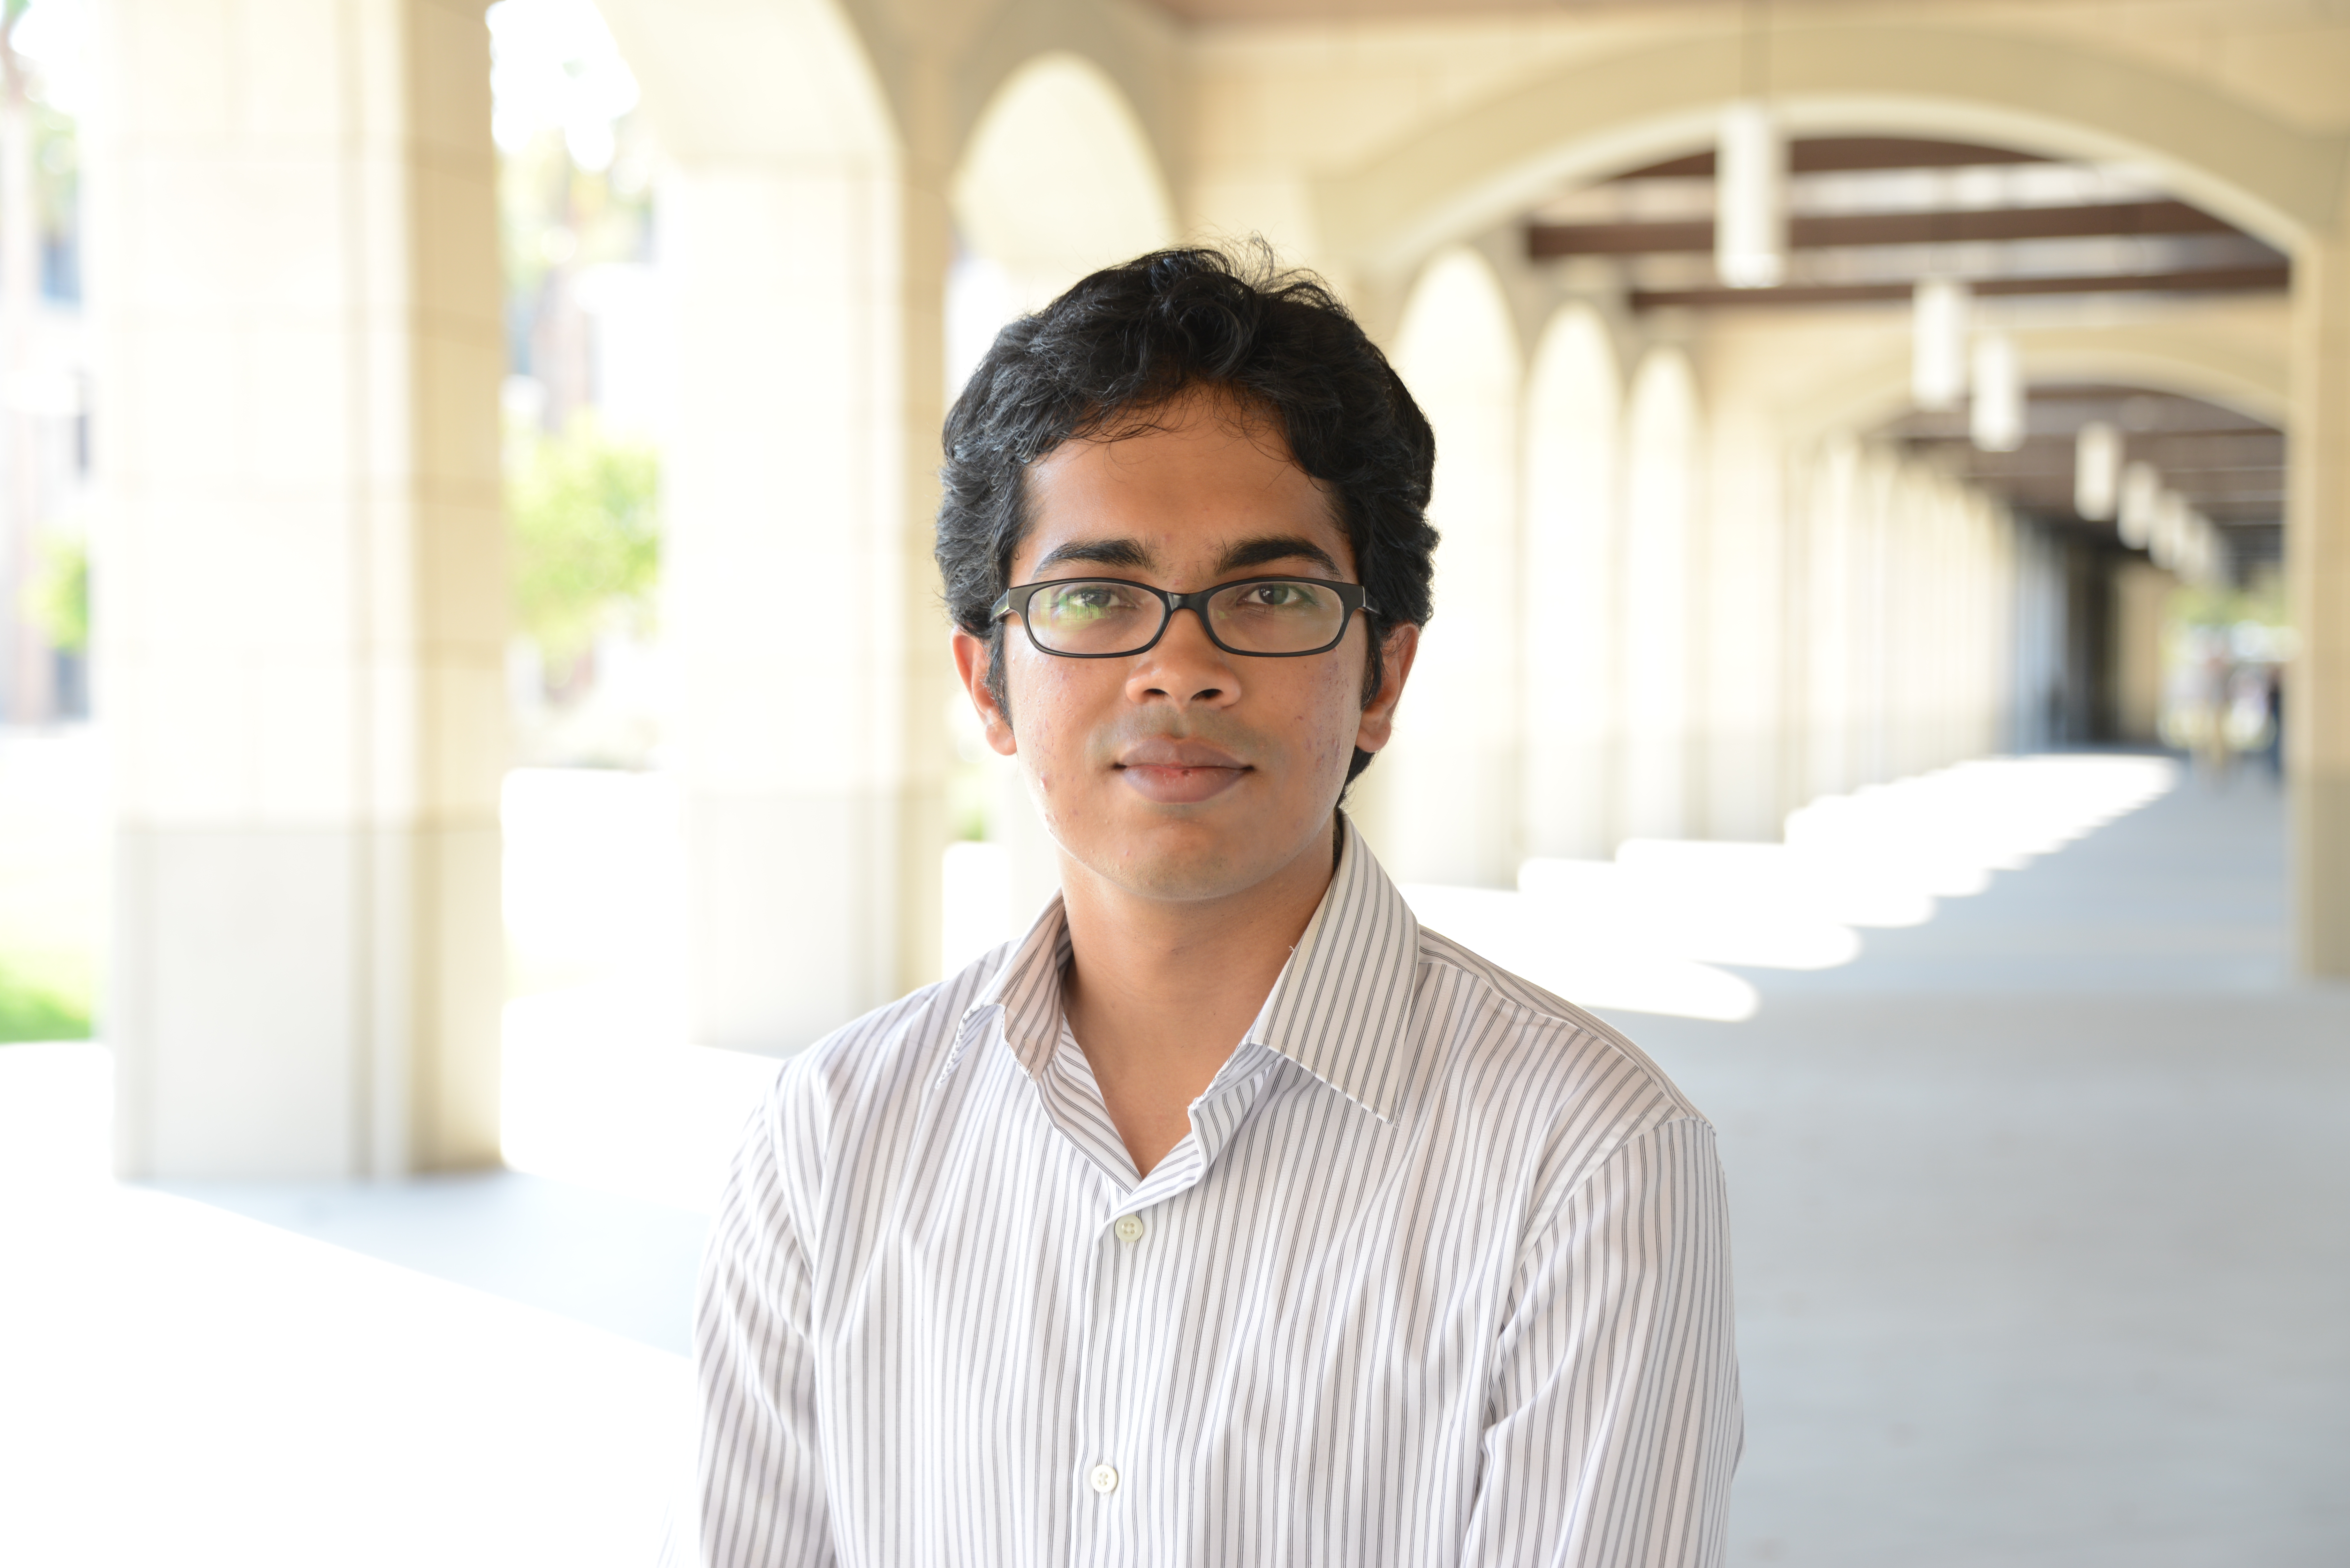
\includegraphics[width=.9\textwidth,height=.9\textwidth,keepaspectratio]{student1.jpg}
	       \end{figure}
	      Materials Science and Engineering
	     \end{column}
		\begin{column}{0.5\textwidth}
		\begin{itemize}
		\setlength\itemsep{1em}
		\item Pune, India. Indian Institute of Technology, Bombay
		\item Solar Energy and Hydrogen Storage
		\item Read, Listen to Music, Hike, Bike
		\end{itemize}
		\end{column}
	\end{columns}
	\end{frame}